% !TeX root = ../dokumentation.tex

\appendixtoc
\renewcommand\thechapter{\Alph{chapter}}
\setcounter{chapter}{0}

% \pagebreak
% \includepdf[pages=-,scale=.9,pagecommand={}]{Aufgabenstellung.pdf} 
% PDF um 10% verkleinert einbinden --> Kopf- und Fußzeile  werden so korrekt dargestellt. Die Option `pages' ermöglicht es, eine bestimmte Sequenz von Seiten (z.B. 2-10 oder `-' für alle Seiten) auszuwählen.
% \pagebreak
%\includepdf[pages=-,scale=.8,pagecommand=\section*{A. eventGenerator.py}]{../appendix/eventGenerator.py.pdf}
%\includepdf[pages=-,scale=.8,pagecommand=\section*{B. sendEvents.py}]{../appendix/sendEvents.py.pdf}


%%%%%%%%%%%%%%%%%%%%%%%%%%%%%%%%%%%%%%%%%%%%%%%%%%%%%
\chapter{Grafiken}

%%%%%%%%%%%%%%%%%%%%%%%%%%%%%%%%%%%%%%%%%%%%%%%%%%%%%
\chapter{Tabellenwerke}

%%%%%%%%%%%%%%%%%%%%%%%%%%%%%%%%%%%%%%%%%%%%%%%%%%%%%
\chapter{Sonstiges}

% \section{Datenblatt: Titan Grade 5 (3.7165; Ti6Al4V) - HWN Titan GmbH \cite{HWN.2022}}
% \label{section:Titandatenblatt}
% \begin{figure}[h]
%     \centering
%     \includegraphics[width=.73\textwidth]{images/appendix/DatenblattTitanGrade5.png}
% \end{figure}
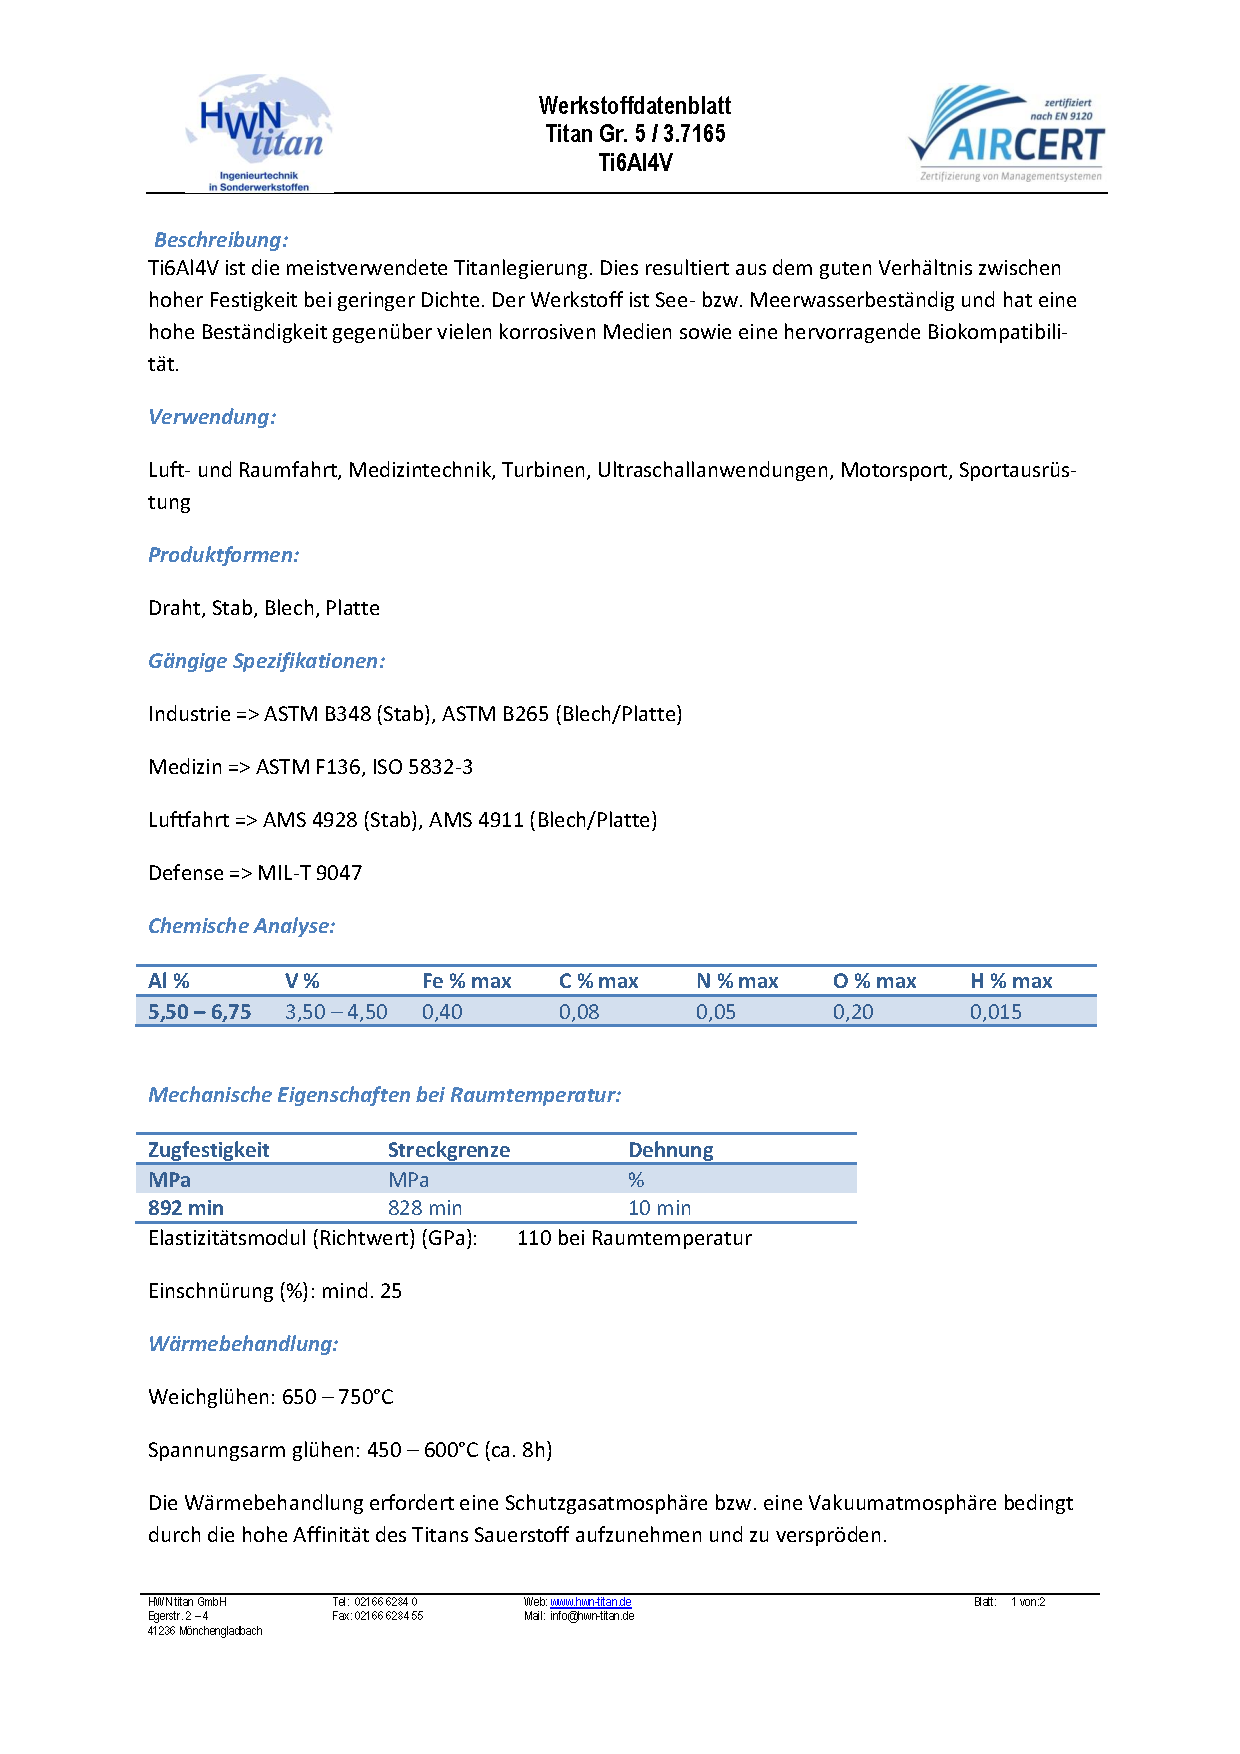
\includepdf[pages=1,scale=.7,pagecommand=\section{Datenblatt: Titan Grade 5 (3.7165; Ti6Al4V) - HWN Titan GmbH}\label{section:Titandatenblatt}]{images/appendix/titan-grade-5-werkstoffdatenblatt.pdf}